\begin{frame}
	\myheading{Module 21.3: Variational autoencoders: (The graphical model perspective)}
\end{frame}


\begin{frame}
	\begin{columns}
		\column{0.4\textwidth}
		\begin{overlayarea}{\textwidth}{\textheight}
			% LHS: figure of Autoencoder with the encoder decoder equations
			\vspace{3pt}
			\tikzstyle{input_neuron}=[circle,draw=black!100,fill=gray!80,thick,minimum size=6mm]
\tikzstyle{hidden_neuron}=[circle,draw=black!100,fill=white!100,thick,minimum size=6mm]
\tikzstyle{output_neuron}=[circle,draw=green!50,fill=green!10,thick,minimum size=6mm]

\tikzstyle{input}=[circle,draw=black!50,fill=black!20,thick,minimum size=6mm]

\begin{center}
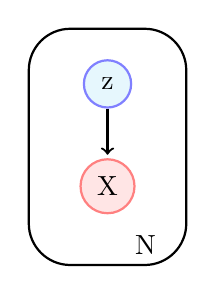
\begin{tikzpicture}
\node [input_neuron] (neuron51) at (7.5,6.5) {X} ;
\node [hidden_neuron] (neuron52) at (7.5,7.8)  {z};
\node[text width=0.1cm] at (7.9,5.75) {N};
\draw[black!100,thick,solid,rounded corners=15pt] (6.5,5.5) rectangle (8.5,8.5);
\draw[thick,->] (7.5,7.48) -- (7.5,6.9);
\end{tikzpicture}
\end{center}


		\end{overlayarea}
		\column{0.6\textwidth}
		\begin{overlayarea}{\textwidth}{\textheight}
			\begin{itemize}[<+->]\justifying
				\item Here we can think of $z$ and $X$ as random variables
				\item We are then interested in the joint probability distribution $P(X,z)$ which factorizes as $P(X,z) = P(z)P(X|z)$
				\item This factorization is natural because we can imagine that the latent variables are fixed first and then the visible variables are drawn based on the latent variables
				\item For example, if we want to draw a digit we could first fix the latent variables:  \textit{the digit, size, angle, thickness, position and so on} and then draw a digit which corresponds to these latent variables
				\item And of course, unlike RBMs, this is a directed graphical model
			\end{itemize}
		\end{overlayarea}
	\end{columns}
\end{frame}


\begin{frame}
	\begin{columns}
		\column{0.4\textwidth}
		\begin{overlayarea}{\textwidth}{\textheight}
			% LHS: same a previous slide?
			\vspace{3pt}
			\tikzstyle{input_neuron}=[circle,draw=black!100,fill=gray!80,thick,minimum size=6mm]
\tikzstyle{hidden_neuron}=[circle,draw=black!100,fill=white!100,thick,minimum size=6mm]
\tikzstyle{output_neuron}=[circle,draw=green!50,fill=green!10,thick,minimum size=6mm]

\tikzstyle{input}=[circle,draw=black!50,fill=black!20,thick,minimum size=6mm]

\begin{center}
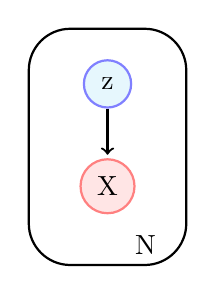
\begin{tikzpicture}
\node [input_neuron] (neuron51) at (7.5,6.5) {X} ;
\node [hidden_neuron] (neuron52) at (7.5,7.8)  {z};
\node[text width=0.1cm] at (7.9,5.75) {N};
\draw[black!100,thick,solid,rounded corners=15pt] (6.5,5.5) rectangle (8.5,8.5);
\draw[thick,->] (7.5,7.48) -- (7.5,6.9);
\end{tikzpicture}
\end{center}

			\vspace{-20pt}

		\end{overlayarea}
		\column{0.6\textwidth}
		\begin{overlayarea}{\textwidth}{\textheight}
			\footnotesize{\begin{itemize}\justifying
				\item<1->Now at inference time, we are given an $X$ (observed variable) and we are interested in finding the most likely assignments of latent variables $z$ which would have resulted in this observation
				\item<2-> Mathematically, we want to find
				\begin{align*}
				P(z|X) = \frac{P(X|z)P(z)}{ P(X)}
				\end{align*}
				\item<3-> This is hard to compute because the LHS contains $P(X)$ which is intractable
				\vspace{-0.1in}
				\begin{align*}
				\hspace{-17em}
					&P(X) = \int P(X|z)P(z) dz\\
					&= \int \int...\int P(X|z_1,z_2, ...,z_n)P(z_1,z_2, ...,z_n) dz_1, ...dz_n
				\end{align*}
				% \vspace{-0.3in}				
				\item<4->  In RBMs, we had a similar integral which we approximated using Gibbs Sampling
				\item<5-> VAEs, on the other hand, cast this into an optimization problem and learn the parameters of the optimization problem
			\end{itemize}}
		\end{overlayarea}
	\end{columns}
\end{frame}


\begin{frame}
	\begin{columns}
		\column{0.4\textwidth}
		\begin{overlayarea}{\textwidth}{\textheight}
			\vspace{3pt}
			\tikzstyle{input_neuron}=[circle,draw=black!100,fill=gray!80,thick,minimum size=6mm]
\tikzstyle{hidden_neuron}=[circle,draw=black!100,fill=white!100,thick,minimum size=6mm]
\tikzstyle{output_neuron}=[circle,draw=green!50,fill=green!10,thick,minimum size=6mm]

\tikzstyle{input}=[circle,draw=black!50,fill=black!20,thick,minimum size=6mm]

\begin{center}
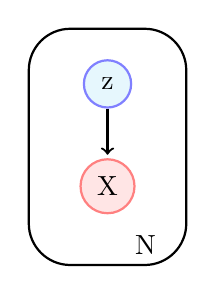
\begin{tikzpicture}
\node [input_neuron] (neuron51) at (7.5,6.5) {X} ;
\node [hidden_neuron] (neuron52) at (7.5,7.8)  {z};
\node[text width=0.1cm] at (7.9,5.75) {N};
\draw[black!100,thick,solid,rounded corners=15pt] (6.5,5.5) rectangle (8.5,8.5);
\draw[thick,->] (7.5,7.48) -- (7.5,6.9);
\end{tikzpicture}
\end{center}

			\vspace{-20pt}
		\end{overlayarea}
		\column{0.6\textwidth}
		\begin{overlayarea}{\textwidth}{\textheight}
			\begin{itemize}[<+->]\justifying
				\item Specifically, in VAEs, we assume that instead of $P(z|X)$ which is intractable, the posterior distribution is given by $Q_\theta(z|X)$
				\item Further, we assume that $Q_\theta(z|X)$ is a Gaussian whose parameters are determined by a neural network 
				$\mu$, $\Sigma = g_\theta(X)$
				\item The parameters of the distribution are thus determined by the parameters $\theta$ of a neural network
				\item Our job then is to learn the parameters of this neural network
			\end{itemize}
		\end{overlayarea}
	\end{columns}
\end{frame}


\begin{frame}
	\begin{columns}
		\column{0.4\textwidth}
		\begin{overlayarea}{\textwidth}{\textheight}
			\vspace{3pt}
			\tikzstyle{input_neuron}=[circle,draw=black!100,fill=gray!80,thick,minimum size=6mm]
\tikzstyle{hidden_neuron}=[circle,draw=black!100,fill=white!100,thick,minimum size=6mm]
\tikzstyle{output_neuron}=[circle,draw=green!50,fill=green!10,thick,minimum size=6mm]

\tikzstyle{input}=[circle,draw=black!50,fill=black!20,thick,minimum size=6mm]

\begin{center}
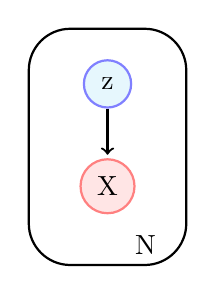
\begin{tikzpicture}
\node [input_neuron] (neuron51) at (7.5,6.5) {X} ;
\node [hidden_neuron] (neuron52) at (7.5,7.8)  {z};
\node[text width=0.1cm] at (7.9,5.75) {N};
\draw[black!100,thick,solid,rounded corners=15pt] (6.5,5.5) rectangle (8.5,8.5);
\draw[thick,->] (7.5,7.48) -- (7.5,6.9);
\end{tikzpicture}
\end{center}

			\vspace{-20pt}
		\end{overlayarea}
		\column{0.6\textwidth}
		\begin{overlayarea}{\textwidth}{\textheight}
			\begin{itemize}\justifying
				\item<1-> But what is the objective function for this neural network
				\item<2-> Well we want the proposed distribution  $Q_\theta(z|X)$ to be as close to the true distribution
				\item<3-> We can capture this using the following objective function
				\begin{align*}
					minimize \hspace{0.2cm}KL(Q_\theta(z|X)||P(z|X))
				\end{align*}
				\item<4-> What are the parameters of the objective function ? \onslide<5->{(they are the parameters of the neural network - we will return back to this again)}
			\end{itemize}
		\end{overlayarea}
	\end{columns}
\end{frame}


\begin{frame}
	%\begin{columns}
	%	\column{0.4\textwidth}
	%	\begin{overlayarea}{\textwidth}{\textheight}
	%	\end{overlayarea}
	%	\column{0.6\textwidth}
	%	\begin{overlayarea}{\textwidth}{\textheight}
	%		\footnotesize{
			\begin{itemize}\justifying
				\item Let us expand the KL divergence term
				\begin{align*}
				D[Q_\theta(z|X)||P(z|X)] \onslide<2->{&= \int Q_\theta(z|X) \log Q_\theta(z|X) dz - \int Q_\theta(z|X) \log P(z|X) dz\\}
				\onslide<3->{&=  \mathbb{E}_{z\sim Q_\theta(z|X)} [ \log Q_\theta(z|X) - \log P(z|X)]}
				%\onslide<6>{&=  \mathbb{E}_{z\sim Q_\theta(z|X)} [ \log Q_\theta(z|X) - \color{red}\log p(z|X)\color{black}]}
				%\onslide<7->{&=  \mathbb{E}_{z\sim Q_\theta(z|X)} [ \log Q_\theta(z|X) - \log p(z|X)]}
				\end{align*}
				\item<4-> For shorthand we will use $\mathbb{E}_Q = \mathbb{E}_{z\sim Q_\theta(z|X)}$ 
				\item<5-> Substituting $P(z|X) = \frac{P(X|z) P(z)}{P(X)}$, we get
				\begin{align*}
				%\onslide<6->{D[q(z|X)||p(z|X)] &= \mathbb{E}_Q [ \log Q_\theta(z|X) - \color{red}\log p(X|z)\color{black} - \color{red}\log p(z)\color{black} + \color{red}\log P(X)\color{black}]\\}
				\onslide<6->{D[Q_\theta(z|X)||P(z|X)] &= \mathbb{E}_Q [ \log Q_\theta(z|X) - \log P(X|z) - \log P(z) + \log P(X)]\\}
				\onslide<7->{&= \mathbb{E}_Q [ \log Q_\theta(z|X) - \log P(z)] - \mathbb{E}_Q[\log P(X|z)] + \log P(X)\\}
				\onslide<8->{&= D[Q_\theta(z|X) || p(z)] - \mathbb{E}_Q[\log P(X|z)] + \log P(X)}
				\end{align*}
				\begin{align*}
				\onslide<9->{&\therefore \log p(X) = \color{blue} \mathbb{E}_Q[\log P(X|z)] - D [Q_\theta(z|X) || P(z)]+ \color{red}D[Q_\theta(z|X)||P(z|X)]\color{black}}
				\end{align*}
			\end{itemize}
			%}
	%	\end{overlayarea}
	%\end{columns}
\end{frame}

\begin{frame}
			\begin{itemize}[<+->]\justifying
				\item So, we have 
				\begin{align*}
				\log P(X) = \color{blue}\mathbb{E}_Q[\log P(X|z)] - D [Q_\theta(z|X) || P(z)] + \color{red}D[Q_\theta(z|X)||P(z|X)]\color{black}
				\end{align*}
				\item Recall that we are interested in maximizing the log likelihood 					of the data \textit{i.e. } $P(X)$
				\item Since KL divergence (the \textcolor{red}{red} term) is always $>= 0$ we can say that
				\vspace{-0.1cm}
				\begin{align*}
					\color{blue}\mathbb{E}_Q[\log P(X|z)] - D [Q_\theta(z|X) || P(z)] \color{black}<= \log P(X)
				\end{align*}	
				\vspace{-0.5cm}
				\item The quantity on the LHS is thus a lower bound for the quantity that we want to maximize and is knows as the Evidence lower bound (ELBO)
				\item Maximizing this lower bound is the same as maximizing $\log P(X)$ and hence our equivalent objective now becomes
				%\item Notice that we were given $X$ and we were interested in $P(z|X)$
				%\item Given $X$, $\log P(X)$ is a constant and this constant is equal to the \color{blue}blue \color{black} term + the \color{red}red \color{black} term
				%\item We were interested in minimizing the blue term but given this relation (\color{blue}blue\color{black} + \color{red}red\color{black} = constant), minimizing the \color{blue}blue \color{black} term is the same as maximizing the \color{red}red \color{black} term
				%\item Thus our equivalent objective now becomes:
				\vspace{-0.1cm}
				\begin{align*}
				maximize \hspace{0.2cm}\mathbb{E}_Q[\log P(X|z)] - D [Q_\theta(z|X) || P(z)]
				\end{align*}
				\vspace{-0.5cm}
				%\item This is called the Evidence Lower Bound (ELBO)
				\item And, this method of learning parameters of probability distributions associated with graphical models using optimization (by maximizing ELBO) is called variational inference
				\item Why is this any easier? It is easy because of certain assumptions that we make as discussed on the next slide
			\end{itemize}
\end{frame}


\begin{frame}
	\begin{columns}
		\column{0.4\textwidth}
		\begin{overlayarea}{\textwidth}{\textheight}
		% LHS: show diagram of VAE with q_\theta(z|X) and p_\theta(X|z)
		\vspace{1cm}
		\tikzstyle{input_neuron}=[circle,draw=red!50,fill=red!10,thick,minimum size=6mm]
\tikzstyle{hidden_neuron}=[circle,draw=blue!50,fill=cyan!10,thick,minimum size=6mm]
\tikzstyle{output_neuron}=[circle,draw=green!50,fill=green!10,thick,minimum size=6mm]

\tikzstyle{input}=[circle,draw=black!50,fill=black!20,thick,minimum size=6mm]

\begin{center}
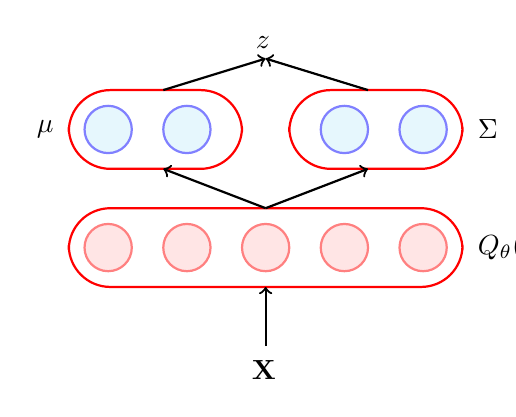
\begin{tikzpicture}

\node [input_neuron] (neuron01) at (6.5,4.5) {};
\node [input_neuron] (neuron02) at (7.5,4.5){};
\node [input_neuron] (neuron03) at (8.5,4.5) {};
\node [input_neuron] (neuron04) at (9.5,4.5) {};
\node [input_neuron] (neuron05) at (10.5,4.5) {};
\node [hidden_neuron] (neuron51) at (6.5,6) {} ;
\node [hidden_neuron] (neuron52) at (7.5,6)  {};
\node [hidden_neuron] (neuron53) at (9.5,6)  {};
\node [hidden_neuron] (neuron54) at (10.5,6)  {};

% \node [output_neuron] (neuron11) at (6.5,7.5)  {};
% \node [output_neuron] (neuron12) at (7.5,7.5)  {};
% \node [output_neuron] (neuron13) at (8.5,7.5)  {};
% \node [output_neuron] (neuron14) at (9.5,7.5)  {};
% \node [output_neuron] (neuron15) at (10.5,7.5)  {};

%\node[text width=0.01cm] at (11.2,4.5) {$\mathbf{X}$};
\node[text width=0.01cm] at (8.33,2.95) {$\mathbf{X}$};
\node[text width=0.01cm] at (8.38,7.1) {$z$};
\node[text width=0.01cm] at (11.2,4.5) {$Q_\theta(z|X)$};
% \node[text width=0.007cm] at (7.7,5.25) {$W$};
\node[text width=0.01cm] at (11.2,6) {$\Sigma$};
\node[text width=0.01cm] at (5.6,6) {$\mu$};
% \node[text width=0.007cm] at (7.7,6.75) {$W^*$};
% \node[text width=0.01cm] at (11.2,7.5) {$\mathbf{\hat{x}_i}$};

\draw[red!100,thick,solid,rounded corners=15pt] (6,4) rectangle (11,5);
\draw[red!100,thick,solid,rounded corners=15pt] (6,5.5) rectangle (8.2,6.5);
\draw[red!100,thick,solid,rounded corners=15pt] (8.8,5.5) rectangle (11,6.5);
% \draw[red!100,thick,solid,rounded corners=15pt] (6,7) rectangle (11,8);



\draw[thick,->] (8.5,5) -- (7.2,5.5);

\draw[thick,->] (8.5,5) -- (9.8,5.5);

\draw[thick,->] (8.5,3.25) -- (8.5,4);

\draw[thick,->] (7.2,6.5) -- (8.5,6.9);

\draw[thick,->] (9.8,6.5) -- (8.5,6.9);

% \draw[thick,->] (7.2,6.5) -- (8.5,7);

% \draw[thick,->] (9.8,6.5) -- (8.5,7);


\end{tikzpicture}
\end{center}

		\end{overlayarea}
		\column{0.6\textwidth}
		\begin{overlayarea}{\textwidth}{\textheight}
			\footnotesize{\begin{itemize}[<+->]\justifying
				\item First we will just reintroduce the parameters in the equation to make things explicit
				\begin{align*}
				maximize \hspace{0.2cm}\mathbb{E}_Q[\log P_\phi(X|z)] - D [Q_\theta(z|X) || P(z)]
				\end{align*}
				\item At training time, we are interested in learning  the parameters $\theta$ which maximize the above for every training example $(x_i \in \{x_i\}_{i=1}^N)$
				\item So our total objective function is
				\begin{align*}
				\underset{\theta}{maximize} \sum_{i=1}^N &\mathbb{E}_Q[\log P_\phi(X=x_i|z)] \\
				&- D [Q_\theta(z|X=x_i) || P(z)]
				\end{align*}
				\item We will shorthand $P(X=x_i)$ as $P(x_i)$
				\item However, we will assume that we are using stochastic gradient descent so we need to deal with only one of the terms in the summation corresponding to the current training example
			\end{itemize}}
		\end{overlayarea}
	\end{columns}
\end{frame}

\begin{frame}
	\begin{columns}
		\column{0.4\textwidth}
		\begin{overlayarea}{\textwidth}{\textheight}
		% LHS: same as above
		\vspace{1cm}
		\tikzstyle{input_neuron}=[circle,draw=red!50,fill=red!10,thick,minimum size=6mm]
\tikzstyle{hidden_neuron}=[circle,draw=blue!50,fill=cyan!10,thick,minimum size=6mm]
\tikzstyle{output_neuron}=[circle,draw=green!50,fill=green!10,thick,minimum size=6mm]

\tikzstyle{input}=[circle,draw=black!50,fill=black!20,thick,minimum size=6mm]

\begin{center}
\scalebox{0.7}{
\begin{tikzpicture}

\node [input_neuron] (neuron01) at (6.5,4.5) {};
\node [input_neuron] (neuron02) at (7.5,4.5){};
\node [input_neuron] (neuron03) at (8.5,4.5) {};
\node [input_neuron] (neuron04) at (9.5,4.5) {};
\node [input_neuron] (neuron05) at (10.5,4.5) {};
\node [hidden_neuron] (neuron51) at (6.5,6) {} ;
\node [hidden_neuron] (neuron52) at (7.5,6)  {};
\node [hidden_neuron] (neuron53) at (9.5,6)  {};
\node [hidden_neuron] (neuron54) at (10.5,6)  {};

\node [input_neuron] (neuron11) at (6.5,11)  {};
\node [input_neuron] (neuron12) at (7.5,11)  {};
\node [input_neuron] (neuron13) at (8.5,11)  {};
\node [input_neuron] (neuron14) at (9.5,11)  {};
\node [input_neuron] (neuron15) at (10.5,11)  {};

\node [ellipse,draw=red!50,fill=red!10,thick] (neuron16) at (8.5,8)  {Sample};

\node [] (neuron17) at (8.3,8.6)  {$z$};

\node[text width=0.01cm] at (8.3,3.3) {$\mathbf{X_i}$};
% \node[text width=0.007cm] at (7.7,5.25) {$\theta$};
\node[text width=0.007cm] at (11.2,4.5) {$Q_\theta(z|X)$};
\node[text width=0.01cm] at (11.2,6) {$\Sigma$};
\node[text width=0.01cm] at (5.6,6) {$\mu$};
% \node[text width=0.01cm] at (10.7,6) {$\mathbf{z}$};
% \node[text width=0.007cm] at (7.7,6.75) {$W^*$};
\node[text width=0.007cm] at (11.2,11) {$P_\phi(X|z)$};
\node[text width=0.01cm] at (8.3,12.2) {$\mathbf{\hat{X}_i}$};

\draw[red!100,thick,solid,rounded corners=15pt] (6,4) rectangle (11,5);
% \draw[red!100,thick,solid,rounded corners=15pt] (6.5,5.5) rectangle (10.5,6.5);
\draw[red!100,thick,solid,rounded corners=15pt] (6,5.5) rectangle (8.2,6.5);
\draw[red!100,thick,solid,rounded corners=15pt] (8.8,5.5) rectangle (11,6.5);
\draw[red!100,thick,solid,rounded corners=15pt] (6,10.5) rectangle (11,11.5);


\draw[thick,->] (8.5,3.5) -- (8.5,4);
\only<3->{\draw[line width=1mm,->,red!100] (8.5,3.5) -- (8.5,4);}

\draw[thick,->] (8.5,5) -- (7.2,5.5);
\only<4->{\draw[line width=1mm,->,red!100] (8.5,5) -- (7.2,5.5);}

\draw[thick,->] (8.5,5) -- (9.8,5.5);
\only<4->{\draw[line width=1mm,->,red!100] (8.5,5) -- (9.8,5.5);}

\draw[thick,->] (7.2,6.5) -- (8.5,7.55);

\draw[thick,->] (9.8,6.5) -- (8.5,7.55);

\draw[thick,->] (8.5,8.45) -- (8.5,10.5);

\draw[thick,->] (8.5,11.5) -- (8.5,12);

\end{tikzpicture}}
\end{center}

		\end{overlayarea}
		\column{0.6\textwidth}
		\begin{overlayarea}{\textwidth}{\textheight}
			\footnotesize{\begin{itemize}[<+->]\justifying
				\item So our objective function w.r.t. one example is 
				\vspace{-0.1cm}
				\begin{align*}
				\underset{\theta}{maximize}  \hspace{0.2cm}\mathbb{E}_Q[\log P_\phi(x_i|z)] - D [Q_\theta(z|x_i) || P(z)]
				\end{align*}
				\vspace{-0.3cm}
				\item Now, first we will do a forward prop through the encoder using $X_i$ 
				% (show animation on LHS figure) 
				and compute $\mu(X)$ and $\Sigma (X)$
				\item<5-> The second term in the above objective function is the difference between two normal distribution $\mathcal{N}(\mu(X), \Sigma(X))$ and $\mathcal{N}(0, I)$
				\item<6-> With some simple trickery you can show that this term reduces to the following expression (Seep proof here)
				\begin{align*}
				&D[\mathcal{N}(\mu(X),\Sigma(X))||\mathcal{N}(0,I)] \\
				&=\frac{1}{2}(tr(\Sigma(X))+(\mu(X))^T[\mu(X))-k-\log det(\Sigma(X))]
				\end{align*}
				where $k$ is the dimensionality of the latent variables 
				% : a link to the derivation which we can add later
				\item<7-> This term can be computed easily because we have already computed $\mu(X)$ and $\Sigma(X)$ in the forward pass 
			\end{itemize}}
		\end{overlayarea}
	\end{columns}
\end{frame}

\begin{frame}
	\begin{columns}
		\column{0.4\textwidth}
		\begin{overlayarea}{\textwidth}{\textheight}
% LHS: same as above (put the objective function below the figure)
		\vspace{1cm}
		\tikzstyle{input_neuron}=[circle,draw=red!50,fill=red!10,thick,minimum size=6mm]
\tikzstyle{hidden_neuron}=[circle,draw=blue!50,fill=cyan!10,thick,minimum size=6mm]
\tikzstyle{output_neuron}=[circle,draw=green!50,fill=green!10,thick,minimum size=6mm]

\tikzstyle{input}=[circle,draw=black!50,fill=black!20,thick,minimum size=6mm]

\begin{center}
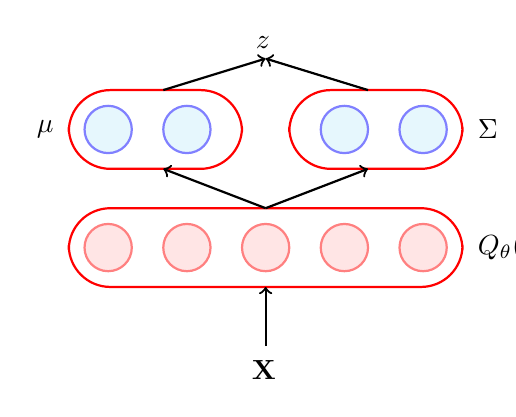
\begin{tikzpicture}

\node [input_neuron] (neuron01) at (6.5,4.5) {};
\node [input_neuron] (neuron02) at (7.5,4.5){};
\node [input_neuron] (neuron03) at (8.5,4.5) {};
\node [input_neuron] (neuron04) at (9.5,4.5) {};
\node [input_neuron] (neuron05) at (10.5,4.5) {};
\node [hidden_neuron] (neuron51) at (6.5,6) {} ;
\node [hidden_neuron] (neuron52) at (7.5,6)  {};
\node [hidden_neuron] (neuron53) at (9.5,6)  {};
\node [hidden_neuron] (neuron54) at (10.5,6)  {};

% \node [output_neuron] (neuron11) at (6.5,7.5)  {};
% \node [output_neuron] (neuron12) at (7.5,7.5)  {};
% \node [output_neuron] (neuron13) at (8.5,7.5)  {};
% \node [output_neuron] (neuron14) at (9.5,7.5)  {};
% \node [output_neuron] (neuron15) at (10.5,7.5)  {};

%\node[text width=0.01cm] at (11.2,4.5) {$\mathbf{X}$};
\node[text width=0.01cm] at (8.33,2.95) {$\mathbf{X}$};
\node[text width=0.01cm] at (8.38,7.1) {$z$};
\node[text width=0.01cm] at (11.2,4.5) {$Q_\theta(z|X)$};
% \node[text width=0.007cm] at (7.7,5.25) {$W$};
\node[text width=0.01cm] at (11.2,6) {$\Sigma$};
\node[text width=0.01cm] at (5.6,6) {$\mu$};
% \node[text width=0.007cm] at (7.7,6.75) {$W^*$};
% \node[text width=0.01cm] at (11.2,7.5) {$\mathbf{\hat{x}_i}$};

\draw[red!100,thick,solid,rounded corners=15pt] (6,4) rectangle (11,5);
\draw[red!100,thick,solid,rounded corners=15pt] (6,5.5) rectangle (8.2,6.5);
\draw[red!100,thick,solid,rounded corners=15pt] (8.8,5.5) rectangle (11,6.5);
% \draw[red!100,thick,solid,rounded corners=15pt] (6,7) rectangle (11,8);



\draw[thick,->] (8.5,5) -- (7.2,5.5);

\draw[thick,->] (8.5,5) -- (9.8,5.5);

\draw[thick,->] (8.5,3.25) -- (8.5,4);

\draw[thick,->] (7.2,6.5) -- (8.5,6.9);

\draw[thick,->] (9.8,6.5) -- (8.5,6.9);

% \draw[thick,->] (7.2,6.5) -- (8.5,7);

% \draw[thick,->] (9.8,6.5) -- (8.5,7);


\end{tikzpicture}
\end{center}

		\end{overlayarea}
		\column{0.6\textwidth}
		\begin{overlayarea}{\textwidth}{\textheight}
			\begin{itemize}[<+->]\justifying
				\item Now let us look at the other term in the objective function
				\begin{align*}
				\sum_{i=1}^n \mathbb{E}_Q[\log P_\phi(X|z)]
				\end{align*}
				\item This is again an expectation and hence intractable (integral over $z$)
				\item In VAEs, we approximate this with a single $z$ sampled from $\mathcal{N}(\mu(X), \Sigma(X))$ 
				%(in the LHS show that we are sampling from N(\mu(X), \Sigma(X)) )
				
				% E \approx point estimate
				\item Hence this term is also easy to compute (of course it is a nasty approximation but we will live with it!)
			\end{itemize}
		\end{overlayarea}
	\end{columns}
\end{frame}

\begin{frame}
	\begin{columns}
		\column{0.4\textwidth}
		\begin{overlayarea}{\textwidth}{\textheight}
% LHS: same as above (put the objective function below the figure)
		\vspace{1cm}
		\tikzstyle{input_neuron}=[circle,draw=red!50,fill=red!10,thick,minimum size=6mm]
\tikzstyle{hidden_neuron}=[circle,draw=blue!50,fill=cyan!10,thick,minimum size=6mm]
\tikzstyle{output_neuron}=[circle,draw=green!50,fill=green!10,thick,minimum size=6mm]

\tikzstyle{input}=[circle,draw=black!50,fill=black!20,thick,minimum size=6mm]

\begin{center}
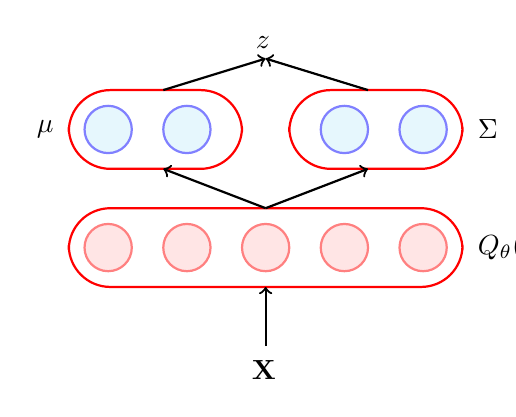
\begin{tikzpicture}

\node [input_neuron] (neuron01) at (6.5,4.5) {};
\node [input_neuron] (neuron02) at (7.5,4.5){};
\node [input_neuron] (neuron03) at (8.5,4.5) {};
\node [input_neuron] (neuron04) at (9.5,4.5) {};
\node [input_neuron] (neuron05) at (10.5,4.5) {};
\node [hidden_neuron] (neuron51) at (6.5,6) {} ;
\node [hidden_neuron] (neuron52) at (7.5,6)  {};
\node [hidden_neuron] (neuron53) at (9.5,6)  {};
\node [hidden_neuron] (neuron54) at (10.5,6)  {};

% \node [output_neuron] (neuron11) at (6.5,7.5)  {};
% \node [output_neuron] (neuron12) at (7.5,7.5)  {};
% \node [output_neuron] (neuron13) at (8.5,7.5)  {};
% \node [output_neuron] (neuron14) at (9.5,7.5)  {};
% \node [output_neuron] (neuron15) at (10.5,7.5)  {};

%\node[text width=0.01cm] at (11.2,4.5) {$\mathbf{X}$};
\node[text width=0.01cm] at (8.33,2.95) {$\mathbf{X}$};
\node[text width=0.01cm] at (8.38,7.1) {$z$};
\node[text width=0.01cm] at (11.2,4.5) {$Q_\theta(z|X)$};
% \node[text width=0.007cm] at (7.7,5.25) {$W$};
\node[text width=0.01cm] at (11.2,6) {$\Sigma$};
\node[text width=0.01cm] at (5.6,6) {$\mu$};
% \node[text width=0.007cm] at (7.7,6.75) {$W^*$};
% \node[text width=0.01cm] at (11.2,7.5) {$\mathbf{\hat{x}_i}$};

\draw[red!100,thick,solid,rounded corners=15pt] (6,4) rectangle (11,5);
\draw[red!100,thick,solid,rounded corners=15pt] (6,5.5) rectangle (8.2,6.5);
\draw[red!100,thick,solid,rounded corners=15pt] (8.8,5.5) rectangle (11,6.5);
% \draw[red!100,thick,solid,rounded corners=15pt] (6,7) rectangle (11,8);



\draw[thick,->] (8.5,5) -- (7.2,5.5);

\draw[thick,->] (8.5,5) -- (9.8,5.5);

\draw[thick,->] (8.5,3.25) -- (8.5,4);

\draw[thick,->] (7.2,6.5) -- (8.5,6.9);

\draw[thick,->] (9.8,6.5) -- (8.5,6.9);

% \draw[thick,->] (7.2,6.5) -- (8.5,7);

% \draw[thick,->] (9.8,6.5) -- (8.5,7);


\end{tikzpicture}
\end{center}

		\end{overlayarea}
		\column{0.6\textwidth}
		\begin{overlayarea}{\textwidth}{\textheight}
			\begin{itemize}[<+->]\justifying
				\item Further, as usual, we need to assume some parametric form for $P(X|z)$
				\item For example, if we assume that $P(X|z)$ is a Gaussian with mean $\mu(z)$ and variance $I$ then
				\vspace{-0.7cm}
				\begin{align*}
				\log P(X = X_i|z) = C - \frac{1}{2}||X_i - \mu(z)||^2
				\end{align*}
				\vspace{-0.7cm}
				\item $\mu(z)$ in turn is a function of the parameters of the decoder and can be written as $f_\phi(z)$
				\vspace{-0.4cm}
				\onslide<4->{\begin{align*}
				\log P(X = X_i|z) = C - \frac{1}{2} ||X_i - f_\phi(z)||^2
				\end{align*}}
				\vspace{-0.6cm}
				\item<5-> Our effective objective function thus becomes
				\footnotesize{\begin{align*}
					\underset{\theta,\phi}{minimize}\hspace{0.2cm} & \sum_{n=1}^N \bigg[\frac{1}{2}(tr(\Sigma(X_i))+(\mu(X_i))^T[\mu(X_i))-k\\
					& -\log det(\Sigma(X_i))] + ||X_i - f_\phi(z)||^2 \bigg]
				\end{align*}}
			\end{itemize}
		\end{overlayarea}
	\end{columns}
\end{frame}

\begin{frame}
	\begin{columns}
		\column{0.4\textwidth}
		\begin{overlayarea}{\textwidth}{\textheight}
% LHS: same as above (put the objective function below the figure)
		\vspace{1cm}
		\tikzstyle{input_neuron}=[circle,draw=red!50,fill=red!10,thick,minimum size=6mm]
\tikzstyle{hidden_neuron}=[circle,draw=blue!50,fill=cyan!10,thick,minimum size=6mm]
\tikzstyle{output_neuron}=[circle,draw=green!50,fill=green!10,thick,minimum size=6mm]

\tikzstyle{input}=[circle,draw=black!50,fill=black!20,thick,minimum size=6mm]

\begin{center}
\scalebox{0.7}{
\begin{tikzpicture}

\node [input_neuron] (neuron01) at (6.5,4.5) {};
\node [input_neuron] (neuron02) at (7.5,4.5){};
\node [input_neuron] (neuron03) at (8.5,4.5) {};
\node [input_neuron] (neuron04) at (9.5,4.5) {};
\node [input_neuron] (neuron05) at (10.5,4.5) {};
\node [hidden_neuron] (neuron51) at (6.5,6) {} ;
\node [hidden_neuron] (neuron52) at (7.5,6)  {};
\node [hidden_neuron] (neuron53) at (9.5,6)  {};
\node [hidden_neuron] (neuron54) at (10.5,6)  {};

\node [input_neuron] (neuron11) at (6.5,11)  {};
\node [input_neuron] (neuron12) at (7.5,11)  {};
\node [input_neuron] (neuron13) at (8.5,11)  {};
\node [input_neuron] (neuron14) at (9.5,11)  {};
\node [input_neuron] (neuron15) at (10.5,11)  {};

\only<1-4>{\node [ellipse,draw=red!50,fill=red!10,thick] (neuron16) at (8.5,8)  {Sample};}
\only<5->{\node [line width= 1mm, ellipse,draw=red!80,fill=red!10] (neuron16) at (8.5,8)  {\textbf{\textcolor{blue}{Sample}}};}

\node [] (neuron17) at (8.3,8.6)  {$z$};

\node[text width=0.01cm] at (8.3,3.3) {$\mathbf{X_i}$};
% \node[text width=0.007cm] at (7.7,5.25) {$\theta$};
\node[text width=0.007cm] at (11.2,4.5) {$Q_\theta(z|X)$};
\node[text width=0.01cm] at (11.2,6) {$\Sigma$};
\node[text width=0.01cm] at (5.6,6) {$\mu$};
% \node[text width=0.01cm] at (10.7,6) {$\mathbf{z}$};
% \node[text width=0.007cm] at (7.7,6.75) {$W^*$};
\node[text width=0.007cm] at (11.2,11) {$P_\phi(X|z)$};
\node[text width=0.01cm] at (8.3,12.2) {$\mathbf{\hat{X}_i}$};

\draw[red!100,thick,solid,rounded corners=15pt] (6,4) rectangle (11,5);
% \draw[red!100,thick,solid,rounded corners=15pt] (6.5,5.5) rectangle (10.5,6.5);
\draw[red!100,thick,solid,rounded corners=15pt] (6,5.5) rectangle (8.2,6.5);
\draw[red!100,thick,solid,rounded corners=15pt] (8.8,5.5) rectangle (11,6.5);
\draw[red!100,thick,solid,rounded corners=15pt] (6,10.5) rectangle (11,11.5);


\draw[thick,->] (8.5,3.5) -- (8.5,4);

\draw[thick,->] (8.5,5) -- (7.2,5.5);

\draw[thick,->] (8.5,5) -- (9.8,5.5);

\draw[thick,->] (7.2,6.5) -- (8.5,7.55);

\draw[thick,->] (9.8,6.5) -- (8.5,7.55);

\draw[thick,->] (8.5,8.45) -- (8.5,10.5);

\draw[thick,->] (8.5,11.5) -- (8.5,12);

\end{tikzpicture}}
\end{center}

		\end{overlayarea}
		\column{0.6\textwidth}
		\begin{overlayarea}{\textwidth}{\textheight}
			\begin{itemize}[<+->]\justifying
				\item The above loss can be easily computed and we can update the parameters $\theta$ of the encoder and $\phi$ of decoder using backpropagation
				\item However, there is a catch !
				\item The network is not end to end differentiable because the output $f_\phi(z)$ is not an end to end differentiable function of the input $X$
				\item<4-> Why? \onslide<5->{because after passing X through the network we simply compute  $\mu(X)$ and $\Sigma(X)$ and then sample a $z$ to be fed to the decoder}
				\item<6-> This makes the entire process non-deterministic and hence $f_\phi(z)$ is not a continuous function of the input $X$
			\end{itemize}
		\end{overlayarea}
	\end{columns}
\end{frame}

\begin{frame}
	\begin{columns}
		\column{0.4\textwidth}
		\begin{overlayarea}{\textwidth}{\textheight}
		% LHS: same as above and then change it to show the reparam trick
		\vspace{1cm}
		\only<1-3>{\tikzstyle{input_neuron}=[circle,draw=red!50,fill=red!10,thick,minimum size=6mm]
\tikzstyle{hidden_neuron}=[circle,draw=blue!50,fill=cyan!10,thick,minimum size=6mm]
\tikzstyle{output_neuron}=[circle,draw=green!50,fill=green!10,thick,minimum size=6mm]

\tikzstyle{input}=[circle,draw=black!50,fill=black!20,thick,minimum size=6mm]

\begin{center}
\scalebox{0.7}{
\begin{tikzpicture}

\node [input_neuron] (neuron01) at (6.5,4.5) {};
\node [input_neuron] (neuron02) at (7.5,4.5){};
\node [input_neuron] (neuron03) at (8.5,4.5) {};
\node [input_neuron] (neuron04) at (9.5,4.5) {};
\node [input_neuron] (neuron05) at (10.5,4.5) {};
\node [hidden_neuron] (neuron51) at (6.5,6) {} ;
\node [hidden_neuron] (neuron52) at (7.5,6)  {};
\node [hidden_neuron] (neuron53) at (9.5,6)  {};
\node [hidden_neuron] (neuron54) at (10.5,6)  {};

\node [input_neuron] (neuron11) at (6.5,11)  {};
\node [input_neuron] (neuron12) at (7.5,11)  {};
\node [input_neuron] (neuron13) at (8.5,11)  {};
\node [input_neuron] (neuron14) at (9.5,11)  {};
\node [input_neuron] (neuron15) at (10.5,11)  {};

% \only<1-4>{\node [ellipse,draw=red!50,fill=red!10,thick] (neuron16) at (8.5,8)  {Sample};}
\node [line width= 1mm, ellipse,draw=red!80,fill=red!10] (neuron16) at (8.5,8)  {\textbf{\textcolor{blue}{Sample}}};

\node [] (neuron17) at (8.3,8.6)  {$z$};

\node[text width=0.01cm] at (8.3,3.3) {$\mathbf{X_i}$};
% \node[text width=0.007cm] at (7.7,5.25) {$\theta$};
\node[text width=0.007cm] at (11.2,4.5) {$Q_\theta(z|X)$};
\node[text width=0.01cm] at (11.2,6) {$\Sigma$};
\node[text width=0.01cm] at (5.6,6) {$\mu$};
% \node[text width=0.01cm] at (10.7,6) {$\mathbf{z}$};
% \node[text width=0.007cm] at (7.7,6.75) {$W^*$};
\node[text width=0.007cm] at (11.2,11) {$P_\phi(X|z)$};
\node[text width=0.01cm] at (8.3,12.2) {$\mathbf{\hat{X}_i}$};

\draw[red!100,thick,solid,rounded corners=15pt] (6,4) rectangle (11,5);
% \draw[red!100,thick,solid,rounded corners=15pt] (6.5,5.5) rectangle (10.5,6.5);
\draw[red!100,thick,solid,rounded corners=15pt] (6,5.5) rectangle (8.2,6.5);
\draw[red!100,thick,solid,rounded corners=15pt] (8.8,5.5) rectangle (11,6.5);
\draw[red!100,thick,solid,rounded corners=15pt] (6,10.5) rectangle (11,11.5);


\draw[thick,->] (8.5,3.5) -- (8.5,4);

\draw[thick,->] (8.5,5) -- (7.2,5.5);

\draw[thick,->] (8.5,5) -- (9.8,5.5);

\draw[thick,->] (7.2,6.5) -- (8.5,7.55);

\draw[thick,->] (9.8,6.5) -- (8.5,7.55);

\draw[thick,->] (8.5,8.45) -- (8.5,10.5);

\draw[thick,->] (8.5,11.5) -- (8.5,12);

\end{tikzpicture}}
\end{center}
}
		\only<4->{\tikzstyle{input_neuron}=[circle,draw=red!50,fill=red!10,thick,minimum size=6mm]
\tikzstyle{hidden_neuron}=[circle,draw=blue!50,fill=cyan!10,thick,minimum size=6mm]
\tikzstyle{output_neuron}=[circle,draw=green!50,fill=green!10,thick,minimum size=6mm]

\tikzstyle{input}=[circle,draw=black!50,fill=black!20,thick,minimum size=6mm]

\begin{center}
\scalebox{0.7}{
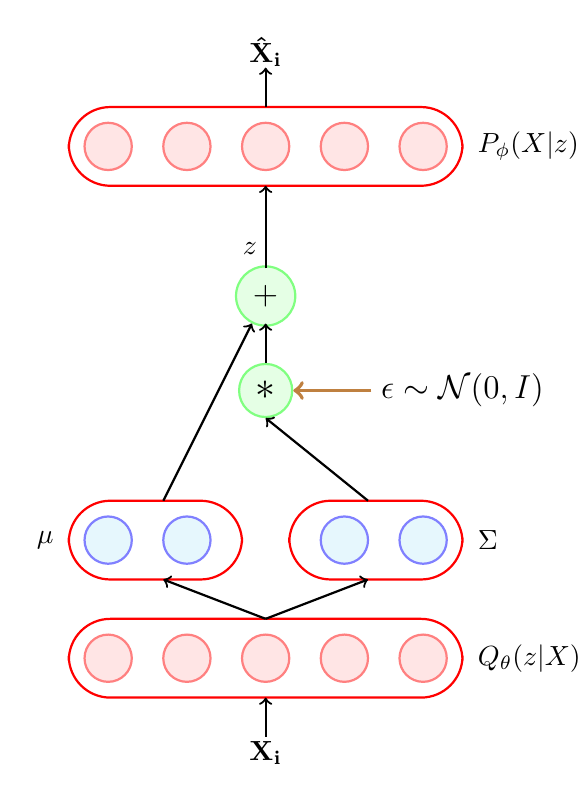
\begin{tikzpicture}

\node [input_neuron] (neuron01) at (6.5,4.5) {};
\node [input_neuron] (neuron02) at (7.5,4.5){};
\node [input_neuron] (neuron03) at (8.5,4.5) {};
\node [input_neuron] (neuron04) at (9.5,4.5) {};
\node [input_neuron] (neuron05) at (10.5,4.5) {};
\node [hidden_neuron] (neuron51) at (6.5,6) {} ;
\node [hidden_neuron] (neuron52) at (7.5,6)  {};
\node [hidden_neuron] (neuron53) at (9.5,6)  {};
\node [hidden_neuron] (neuron54) at (10.5,6)  {};

\node [input_neuron] (neuron11) at (6.5,11)  {};
\node [input_neuron] (neuron12) at (7.5,11)  {};
\node [input_neuron] (neuron13) at (8.5,11)  {};
\node [input_neuron] (neuron14) at (9.5,11)  {};
\node [input_neuron] (neuron15) at (10.5,11)  {};

\node [output_neuron] (neuron17) at (8.5,7.9)  {\Large$\ast$};
\node [output_neuron] (neuron18) at (8.5,9.1)  {\large$+$};
\node [] (neuron19) at (11,7.9)  {\large$\epsilon \sim \mathcal{N}(0,I)$};
\node [] at (8.3,9.7)  {$z$};

\node[text width=0.01cm] at (8.3,3.3) {$\mathbf{X_i}$};
% \node[text width=0.007cm] at (7.7,5.25) {$\theta$};
\node[text width=0.007cm] at (11.2,4.5) {$Q_\theta(z|X)$};
\node[text width=0.01cm] at (11.2,6) {$\Sigma$};
\node[text width=0.01cm] at (5.6,6) {$\mu$};
% \node[text width=0.01cm] at (10.7,6) {$\mathbf{z}$};
% \node[text width=0.007cm] at (7.7,6.75) {$W^*$};
\node[text width=0.007cm] at (11.2,11) {$P_\phi(X|z)$};
\node[text width=0.01cm] at (8.3,12.2) {$\mathbf{\hat{X}_i}$};

\draw[red!100,thick,solid,rounded corners=15pt] (6,4) rectangle (11,5);
% \draw[red!100,thick,solid,rounded corners=15pt] (6.5,5.5) rectangle (10.5,6.5);
\draw[red!100,thick,solid,rounded corners=15pt] (6,5.5) rectangle (8.2,6.5);
\draw[red!100,thick,solid,rounded corners=15pt] (8.8,5.5) rectangle (11,6.5);
\draw[red!100,thick,solid,rounded corners=15pt] (6,10.5) rectangle (11,11.5);

\draw[thick,->] (8.5,3.5) -- (8.5,4);

\draw[thick,->] (8.5,5) -- (7.2,5.5);

\draw[thick,->] (8.5,5) -- (9.8,5.5);

\draw[thick,->] (7.2,6.5) -- (neuron18);

\draw[line width = 0.5mm,->, brown!100] (neuron19) -- (neuron17);

\draw[thick,->] (9.8,6.5) -- (8.5,7.55);

\draw[thick,->] (8.5,8.25) -- (8.5,8.75);

\draw[thick,->] (8.5,9.45) -- (8.5,10.5);

\draw[thick,->] (8.5,11.5) -- (8.5,12);

\end{tikzpicture}}
\end{center}
}
		\end{overlayarea}
		\column{0.6\textwidth}
		\begin{overlayarea}{\textwidth}{\textheight}
			\begin{itemize}[<+->]\justifying
				\item VAEs use a neat trick to get around this problem
				\item This is known as the reparameterization trick wherein we move the process of sampling to an input layer
				\item For 1 dimensional case, given $\mu$ and $\sigma$ we can sample from $\mathcal{N} (\mu, \sigma)$ by first sampling $\epsilon \sim \mathcal{N} (0, 1)$, and then computing 
				\begin{align*}
				z = \mu + \sigma * \epsilon
				\end{align*}
				\item The adjacent figure shows the difference between the original network and the reparamterized network
				\item The randomness in $f_\phi(z)$ is now associated with $\epsilon$ and not $X$ or the parameters of the model
			\end{itemize}
		\end{overlayarea}
	\end{columns}
\end{frame}

\begin{frame}
	\begin{columns}
		\column{0.4\textwidth}
		\begin{overlayarea}{\textwidth}{\textheight}
			\footnotesize{\begin{itemize}[<2->]\justifying
				\item \textbf{Data:} $\{X_i\}_{i=1}^N$
				\item \textbf{Model:} $\hat{X} = f_\phi(\mu(X) + \Sigma(X) \ast \epsilon)$
				\item \textbf{Parameters:} $\theta, \phi$
				\item \textbf{Algorithm:} Gradient descent
				\item \textbf{Objective:} 
				\begin{align*}
					& \sum_{n=1}^N \bigg[\frac{1}{2}(tr(\Sigma(X_i))+(\mu(X_i))^T[\mu(X_i))\\
					& -k-\log det(\Sigma(X_i))] + ||X_i - f_\phi(z)||^2 \bigg]
				\end{align*}
			\end{itemize}}
		\end{overlayarea}
		\column{0.6\textwidth}
		\begin{overlayarea}{\textwidth}{\textheight}
			\begin{itemize}[<+->]\justifying
				\item With that we are done with the process of training VAEs
				\item Specifically, we have described the data, model, parameters, objective function and learning algorithm
				\item Now what happens at test time? We need to consider both \textit{abstraction} and \textit{generation}
				\item In other words we are interested in computing a $z$ given a $X$ as well as in generating a $X$ given a $z$
				\item Let us look at each of these goals
			\end{itemize}
		\end{overlayarea}
	\end{columns}
\end{frame}

\begin{frame}
	\begin{columns}
		\column{0.4\textwidth}
		\begin{overlayarea}{\textwidth}{\textheight}
		\vspace{1cm}
		\tikzstyle{input_neuron}=[circle,draw=red!50,fill=red!10,thick,minimum size=6mm]
\tikzstyle{hidden_neuron}=[circle,draw=blue!50,fill=cyan!10,thick,minimum size=6mm]
\tikzstyle{output_neuron}=[circle,draw=green!50,fill=green!10,thick,minimum size=6mm]

\tikzstyle{input}=[circle,draw=black!50,fill=black!20,thick,minimum size=6mm]

\begin{center}
\scalebox{0.7}{
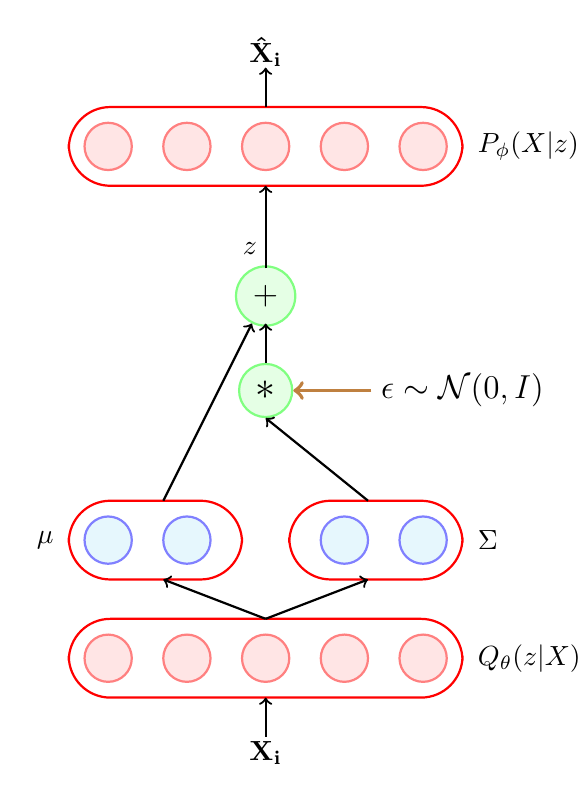
\begin{tikzpicture}

\node [input_neuron] (neuron01) at (6.5,4.5) {};
\node [input_neuron] (neuron02) at (7.5,4.5){};
\node [input_neuron] (neuron03) at (8.5,4.5) {};
\node [input_neuron] (neuron04) at (9.5,4.5) {};
\node [input_neuron] (neuron05) at (10.5,4.5) {};
\node [hidden_neuron] (neuron51) at (6.5,6) {} ;
\node [hidden_neuron] (neuron52) at (7.5,6)  {};
\node [hidden_neuron] (neuron53) at (9.5,6)  {};
\node [hidden_neuron] (neuron54) at (10.5,6)  {};

\node [input_neuron] (neuron11) at (6.5,11)  {};
\node [input_neuron] (neuron12) at (7.5,11)  {};
\node [input_neuron] (neuron13) at (8.5,11)  {};
\node [input_neuron] (neuron14) at (9.5,11)  {};
\node [input_neuron] (neuron15) at (10.5,11)  {};

\node [output_neuron] (neuron17) at (8.5,7.9)  {\Large$\ast$};
\node [output_neuron] (neuron18) at (8.5,9.1)  {\large$+$};
\node [] (neuron19) at (11,7.9)  {\large$\epsilon \sim \mathcal{N}(0,I)$};
\node [] at (8.3,9.7)  {$z$};

\node[text width=0.01cm] at (8.3,3.3) {$\mathbf{X_i}$};
% \node[text width=0.007cm] at (7.7,5.25) {$\theta$};
\node[text width=0.007cm] at (11.2,4.5) {$Q_\theta(z|X)$};
\node[text width=0.01cm] at (11.2,6) {$\Sigma$};
\node[text width=0.01cm] at (5.6,6) {$\mu$};
% \node[text width=0.01cm] at (10.7,6) {$\mathbf{z}$};
% \node[text width=0.007cm] at (7.7,6.75) {$W^*$};
\node[text width=0.007cm] at (11.2,11) {$P_\phi(X|z)$};
\node[text width=0.01cm] at (8.3,12.2) {$\mathbf{\hat{X}_i}$};

\draw[red!100,thick,solid,rounded corners=15pt] (6,4) rectangle (11,5);
% \draw[red!100,thick,solid,rounded corners=15pt] (6.5,5.5) rectangle (10.5,6.5);
\draw[red!100,thick,solid,rounded corners=15pt] (6,5.5) rectangle (8.2,6.5);
\draw[red!100,thick,solid,rounded corners=15pt] (8.8,5.5) rectangle (11,6.5);
\draw[red!100,thick,solid,rounded corners=15pt] (6,10.5) rectangle (11,11.5);

\draw[thick,->] (8.5,3.5) -- (8.5,4);

\draw[thick,->] (8.5,5) -- (7.2,5.5);

\draw[thick,->] (8.5,5) -- (9.8,5.5);

\draw[thick,->] (7.2,6.5) -- (neuron18);

\draw[line width = 0.5mm,->, brown!100] (neuron19) -- (neuron17);

\draw[thick,->] (9.8,6.5) -- (8.5,7.55);

\draw[thick,->] (8.5,8.25) -- (8.5,8.75);

\draw[thick,->] (8.5,9.45) -- (8.5,10.5);

\draw[thick,->] (8.5,11.5) -- (8.5,12);

\end{tikzpicture}}
\end{center}

		\end{overlayarea}
		\column{0.6\textwidth}
		\begin{overlayarea}{\textwidth}{\textheight}
			\textbf{Abstraction}
			\begin{itemize}[<+->]\justifying
				\item After the model parameters are learned we feed a $X$ to the encoder
				\item By doing a forward pass using the learned parameters of the model we compute $\mu(X)$ and $\Sigma(X)$
				\item We then sample a $z$ from the distribution $\mu(X)$ and $\Sigma(X)$ or using the same reparameterization trick
				\item In other words, once we have obtained $\mu(X)$ and $\Sigma(X)$, we first sample $\epsilon \sim \mathcal{N}(\mu(X), \Sigma(X))$ and then compute z 
				\begin{align*}
				z = \mu + \sigma * \epsilon
				\end{align*}
			\end{itemize}
		\end{overlayarea}
	\end{columns}
\end{frame}

\begin{frame}
	\begin{columns}
		\column{0.4\textwidth}
		\begin{overlayarea}{\textwidth}{\textheight}
		\vspace{1cm}
		\tikzstyle{input_neuron}=[circle,draw=red!50,fill=red!10,thick,minimum size=6mm]
\tikzstyle{hidden_neuron}=[circle,draw=blue!50,fill=cyan!10,thick,minimum size=6mm]
\tikzstyle{output_neuron}=[circle,draw=green!50,fill=green!10,thick,minimum size=6mm]

\tikzstyle{input}=[circle,draw=black!50,fill=black!20,thick,minimum size=6mm]

\begin{center}
\scalebox{0.7}{
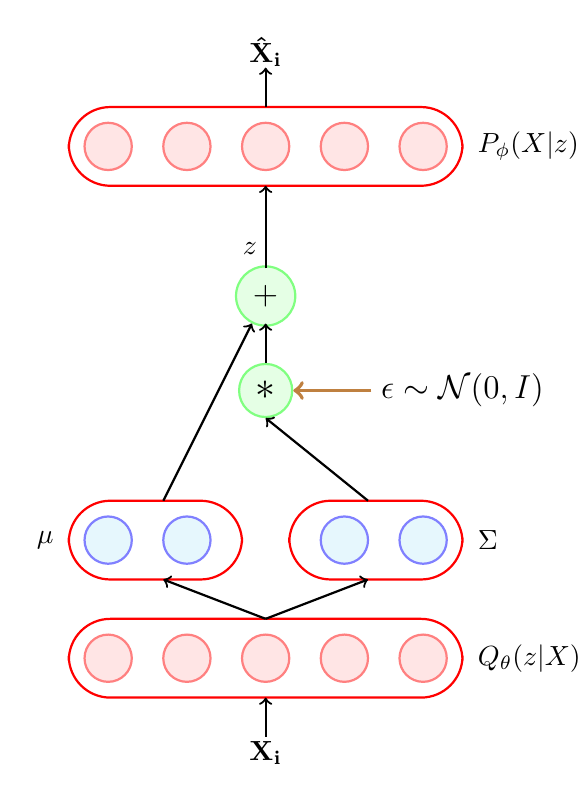
\begin{tikzpicture}

\node [input_neuron] (neuron01) at (6.5,4.5) {};
\node [input_neuron] (neuron02) at (7.5,4.5){};
\node [input_neuron] (neuron03) at (8.5,4.5) {};
\node [input_neuron] (neuron04) at (9.5,4.5) {};
\node [input_neuron] (neuron05) at (10.5,4.5) {};
\node [hidden_neuron] (neuron51) at (6.5,6) {} ;
\node [hidden_neuron] (neuron52) at (7.5,6)  {};
\node [hidden_neuron] (neuron53) at (9.5,6)  {};
\node [hidden_neuron] (neuron54) at (10.5,6)  {};

\node [input_neuron] (neuron11) at (6.5,11)  {};
\node [input_neuron] (neuron12) at (7.5,11)  {};
\node [input_neuron] (neuron13) at (8.5,11)  {};
\node [input_neuron] (neuron14) at (9.5,11)  {};
\node [input_neuron] (neuron15) at (10.5,11)  {};

\node [output_neuron] (neuron17) at (8.5,7.9)  {\Large$\ast$};
\node [output_neuron] (neuron18) at (8.5,9.1)  {\large$+$};
\node [] (neuron19) at (11,7.9)  {\large$\epsilon \sim \mathcal{N}(0,I)$};
\node [] at (8.3,9.7)  {$z$};

\node[text width=0.01cm] at (8.3,3.3) {$\mathbf{X_i}$};
% \node[text width=0.007cm] at (7.7,5.25) {$\theta$};
\node[text width=0.007cm] at (11.2,4.5) {$Q_\theta(z|X)$};
\node[text width=0.01cm] at (11.2,6) {$\Sigma$};
\node[text width=0.01cm] at (5.6,6) {$\mu$};
% \node[text width=0.01cm] at (10.7,6) {$\mathbf{z}$};
% \node[text width=0.007cm] at (7.7,6.75) {$W^*$};
\node[text width=0.007cm] at (11.2,11) {$P_\phi(X|z)$};
\node[text width=0.01cm] at (8.3,12.2) {$\mathbf{\hat{X}_i}$};

\draw[red!100,thick,solid,rounded corners=15pt] (6,4) rectangle (11,5);
% \draw[red!100,thick,solid,rounded corners=15pt] (6.5,5.5) rectangle (10.5,6.5);
\draw[red!100,thick,solid,rounded corners=15pt] (6,5.5) rectangle (8.2,6.5);
\draw[red!100,thick,solid,rounded corners=15pt] (8.8,5.5) rectangle (11,6.5);
\draw[red!100,thick,solid,rounded corners=15pt] (6,10.5) rectangle (11,11.5);

\draw[thick,->] (8.5,3.5) -- (8.5,4);

\draw[thick,->] (8.5,5) -- (7.2,5.5);

\draw[thick,->] (8.5,5) -- (9.8,5.5);

\draw[thick,->] (7.2,6.5) -- (neuron18);

\draw[line width = 0.5mm,->, brown!100] (neuron19) -- (neuron17);

\draw[thick,->] (9.8,6.5) -- (8.5,7.55);

\draw[thick,->] (8.5,8.25) -- (8.5,8.75);

\draw[thick,->] (8.5,9.45) -- (8.5,10.5);

\draw[thick,->] (8.5,11.5) -- (8.5,12);

\end{tikzpicture}}
\end{center}

		\end{overlayarea}
		\column{0.6\textwidth}
		\begin{overlayarea}{\textwidth}{\textheight}
			\textbf{Generation}
			\begin{itemize}[<+->]\justifying
				\item After the model parameters are learned we remove the encoder and feed a $z \sim \mathcal{N}(0,I)$ to the decoder
				\item The decoder will then predict $f_\phi(z)$ and we can draw an $X \sim \mathcal{N}(f_\phi(z), I)$
				\item Why would this work ?
				\item Well, we had trained the model to minimize $D(Q_\theta(z|X) || p(z))$ where $p(z)$ was $\mathcal{N}(0,I)$
				\item If the model is trained well then $Q_\theta(z|X)$ should also become $\mathcal{N}(0,I)$
				\item Hence, if we feed $z \sim \mathcal{N}(0,I)$, it is almost as if we are feeding a $z \sim Q_\theta(z|X)$ and the decoder was indeed trained to produce a good $f_\phi(z)$ from such a $z$
				\item Hence this will work !
			\end{itemize}
		\end{overlayarea}
	\end{columns}
\end{frame}
